\documentclass[12pt]{article}
\usepackage{fullpage}
\usepackage{nopageno}
\usepackage{ifthen}
\usepackage{amsmath}
\usepackage{amssymb}
\usepackage{psfrag} 
\usepackage{graphicx} 
\usepackage{version}
\usepackage{amsthm}
\usepackage{multicol}
%\usepackage{add-copyright}

\excludeversion{solution}

\DeclareMathOperator{\ft}{ft}

\newcommand{\R}{\mathbb{R}}

\title{Take-Home Quiz 8}
\author{Math 131 Section 22}
\date{``Due'' Friday, December 2, 2005}

\newcounter{problem}
\setcounter{problem}{1}

\newenvironment{problem}[1][]
{\begin{flushleft}\hangindent=1em\hangafter=1\noindent\textbf{Problem \arabic{problem}.}
\ifthenelse{\equal{#1}{}}{}{
\textbf{(#1 \ifthenelse{\equal{#1}{1}}{point}{points}).}}
}
{\addtocounter{problem}{1}\end{flushleft}}

\begin{document}
\maketitle

This is the final quiz---and rather than having it due during Reading
Period---which may be forbidden!---this quiz is entirely
\textbf{optional}.  You will receive the full 12 points regardless of
whether you do the quiz or not---but if you do hand it in, I will
comment on your solutions, which might be helpful practice for the
final.

\begin{problem}[4]
You work for a soup company, and you have been given $8\pi$ cubic
inches of soup.  Minimize the surface area of a cylindrical can
holding this volume of soup.
\end{problem}

\begin{problem}[4]
Imagine we live in a world where sheep prefer hexagonal fences (it may
even be this world; I'm not sure if any animals have polygonal
preferences).  You have been given 1200~feet of fence, which you can
divide into four pieces of length $x$ and two pieces of length $y$,
and then attach at 120~degree angles as shown:
\begin{center}
\psfrag{y}{$y$}
\psfrag{x}{$x$}
\psfrag{z}[b][B]{$\sqrt{3} \cdot x$}
\psfrag{w}[b][B]{$x/2$}
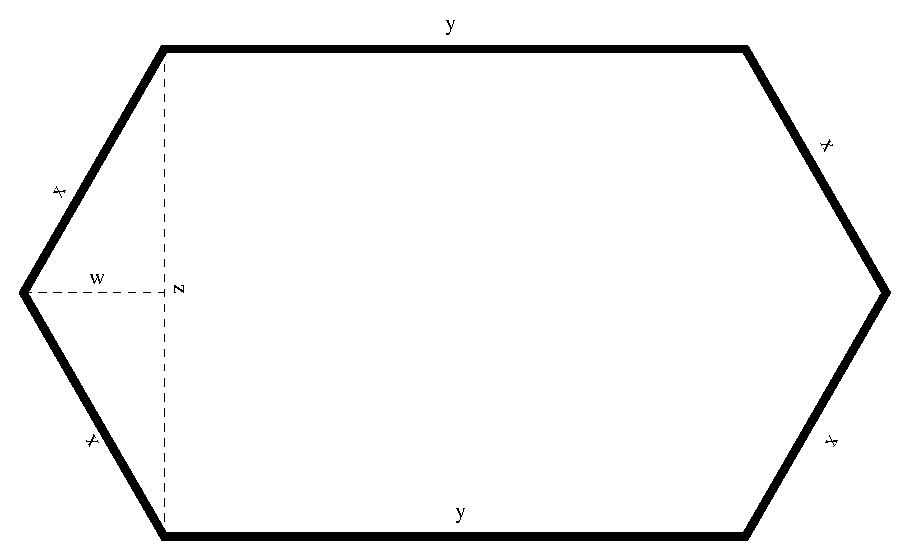
\includegraphics[scale=0.6]{hexagon-field.eps}
\end{center}
What lengths $x$ and $y$ should you choose to maximize the area
enclosed by the hexagon?  I have made some measurements of the dashed
lines (using properties of 30--60--90 triangles) which might help you
in your calculation.
\end{problem}

\pagebreak
\begin{problem}[4]
You are in a canoe (a $k\nu$?), one mile from shore, trying to get to
$Q$, your home, as \textbf{quickly} as possible.  Let $P$ be the point
nearest you on the shore; the distance between $P$ and your home $Q$
is ten miles.

Your plan is to paddle in a straight line (following the dashed line)
to some point $R$ on the shore, and then walk the rest of the way.
You can paddle $3$ miles per hour, and you can walk $4$ miles per
hour.  Describe the best place $R$ to land your canoe by reporting the
distance $x$ between $P$ and $R$.
\begin{center}
\psfrag{shore}{land}
\psfrag{water}{water}
\psfrag{mile}[b][B]{$1\, \mbox{mile}$}
\psfrag{x}[b][B]{$x$}
\psfrag{P}[b][B]{$P$}
\psfrag{Q}[b][B]{$Q$}
\psfrag{R}[b][B]{$R$}
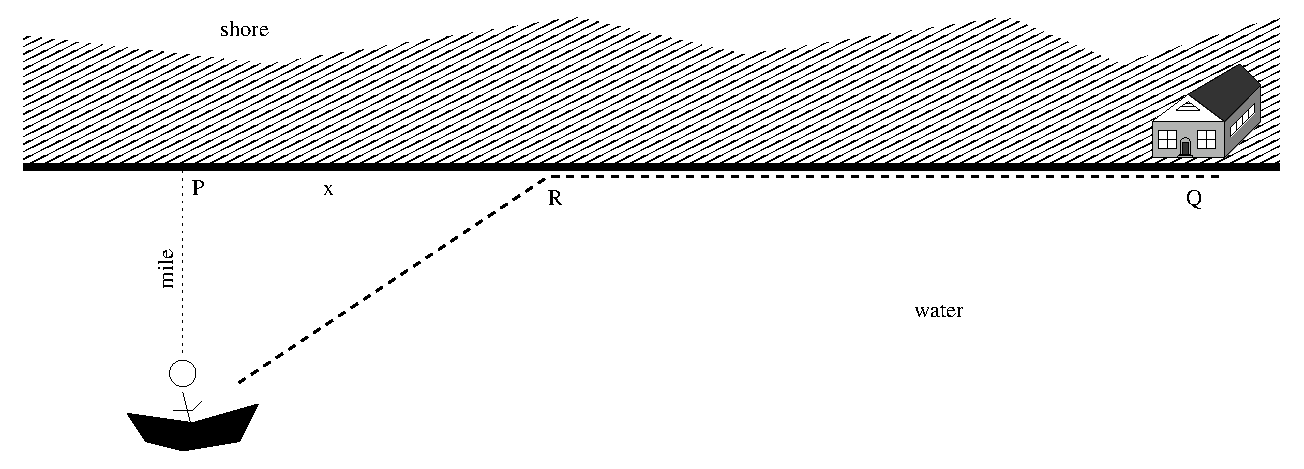
\includegraphics[scale=0.7]{shore.eps}
\end{center}
\end{problem}


\end{document}
